\chapter{Case studies}
\label{chp:case_studies}
% ---------------------------------------------------------------------------------------------------


% ===================================================================================================
\section{A mechanistic emulator: learning the \emph{weir equation}}
% ===================================================================================================

\begin{itemize}
\itemsep0em
  \item present it as a didactic example
  \item use it to compare GP (prior knowledge) with e.g. deep neural networks: how many points can we have?
  \item mention grid convergence study (results go in the appendix)
  \item mention problem with FullSWOF boundary conditions
  \item define well results and methodology
  \item such an emulator can be improved -> modified to compute slope in order to have a given mu value
  \item state all of the goals of the CS: learn weir eq. from simulation, apply curve fitting, get a feeling for simulation accuracy
  \item 
\end{itemize}

As a first case study where to apply the acquired knowledge, it was decided to build an utterly mechanistic emulator.
The main goal of this case study is to try to learn the \emph{weir equation} from simulated data instead of from experimental data.
Here we basically rediscover the way science has always been done, by observing, measuring and trying to find mathematical relationships, with the biggest difference being the fact that the experimental set-up is completely computer built.\\

The \emph{weir equation} computes the discharge $Q$ over a weir as a function of the water depth over the weir itself ($h_w$).
In its simplest form the weir equation can be written as

\begin{equation}
  Q = K\: h_w^{3/2}
\end{equation}

\noindent Where the coefficient $K$ is the only parameter which has to be determined by fitting the model to the data, e.g. by solving the \emph{least squares problem}.

In order to give more physical meaning to the equation and break up the dependencies of the coefficient $K$, the equation can be put under the form

\begin{equation}
  Q = \frac{2}{3}\: \mu\: B_w\: \sqrt{2g}\: h_w^{2/3}
\end{equation}

\noindent Where the coefficient $K$ was decomposed in more contributors: the weir width $B_w$, the gravitational acceleration component $\frac{2}{3}\: \sqrt{2g}$ \noteseb{$\sqrt{2g}$ looks very big} and the coefficient $\mu$, depending on the weir type (broad-crested/sharp-crested) and its particular form.


% ---------------------------------------------------------------------------------------------------
\subsection{Material and methods}
% ---------------------------------------------------------------------------------------------------


% ---------------------------------------------------------------------------------------------------
\subsection{Results and discussion}
% ---------------------------------------------------------------------------------------------------

Present and discuss briefly the results of this toy emulator.


% ---------------------------------------------------------------------------------------------------
%An \textit{early flood warning tool} in an essential component of an \textit{early flood warning system}.
%An early flood warning system has to be understood as an integrated system of tools and plans to detect and respond to flood emergencies \autocite{icimod_early_2018}.
%This can be managed by the community themselves and if designed, implemented and operated correctly can make the difference between tragedy and survival.

%Such systems have already been installed in various endangered regions in the world.
%After the major flooding of July 2014, the city of Altstätten in the canton of St. Gallen made the decision to install one.
%The system installed uses cameras, sensors and level meters to gather data and information about the current situation \autocite{st._galler_tageblatt_altstatten_2017}.
%When the value of certain parameters exceed the given threshold, a dangerous situation is recognized and the alarm signal is sent.

%Three years after the installation of the system an alarm rings in the middle of the night.
%Firemen go immediately into action in order to install temporary measures to fight against the water.
%A couple of hours later the torrent overflows at several points and the city gets flooded.
%Damages are less severe than last time, especially thanks to the temporary measures installed, but possibly they could have been reduced even more.

%Crucial in order to limit the damages is the intervention time before the actual flooding occurs.
%The earlier the dangerous situation can be detected the more time is available to the population and authorities to get ready and set up different types of temporary mitigation measures.
%Systems based on sensors monitoring the evolution of the current situation in the upper part of the catchment are quite reliable but do not allow for long anticipation time.

%Numerical simulations can be run with meteorological forecast data and approximate soil saturation conditions in order to obtain early predictions of the event outcome.
%However, the big advantage of predicting with that much anticipation is partially lost due to the duration of such simulations.
%Accurate meteorological forecasts are available only few hours before the event.
%If the model require several hours to run, which is often the case to obtain accurate predictions for catchments of this extent, then the advantage of being able to run it in advance is canceled.

%A possible solution to this problem is the development of an \emph{early flood warning tool} based on an \emph{ad hoc surrogate model} exploiting the catchment specific behavior.
%This early flood warning tool should be able to recognize if a rain event will generate a channel discharge leading to flooding and if yes within how much time.
%For this scope two different emulators are used.
%The first emulator classifies a rain event based on the forecasted \emph{average rain intensity} and \emph{current soil saturation} into two groups: rain events generating discharge exceeding a chosen threshold ($Q_!$) and rain events not generating discharge exceeding the threshold.
%For events exceeding the threshold a second emulator is developed.
%This predicts the time the rain event will need to produce the threshold discharge $Q_!$ at the outlet of the catchment.
% ---------------------------------------------------------------------------------------------------



% ===================================================================================================
\newpage
\section{An hydrological emulator: estimating the \textit{time-to-peak}}
% ===================================================================================================

With this case study it was decided to address a complex hydrological problem by means of emulation.
The problem we want to solve is estimating the time needed for a channel conveying water from a catchment to reach a certain threshold discharge ($Q_!$) at its outlet as a function of rain intensity and initial soil saturation.

For the experiment a synthetic catchment topography was used, which at first glance can make the case study look very abstract.
In reality the emulator is just exploiting the catchment specific behavior, which is of course different from one catchment to another, but the methodology applied here could be applied to whatever catchment.
The emulator developed here, with the appropriate adjustments, could be exploited as an \emph{early flood warning tool}.

As for the previous example, the simulations were run with the open source software \textit{FullSWOF\_2D-v.1.07.00} \autocite{delestre_fullswof:_2014} \noteseb{put the citation every time that it is mentioned?}, while the input files necessary for the simulations were prepared with \textit{GNU Octave 4.2.1} \autocite{octave_community_gnu_2018} \noteseb{how to cite this?} with the aid of the package \textit{fswof2d}.


% ---------------------------------------------------------------------------------------------------
\subsection{Material and methods}
% ---------------------------------------------------------------------------------------------------

\subsubsection{The synthetic topography}

The topography used represents a catchment of size $\SI{2}{\kilo\meter} \times \SI{2}{\kilo\meter}$ and it is visible in Fig~\ref{fig:topography}.
It is composed of a sloping plane with three Gaussian bumps on the top.
The Gaussian bumps have different heights and widths and generate a \emph{Y-shaped channel} which extends from the upper and left boundary down to the lower boundary.
A paraboloid was added to the plane to promote the accumulation of water in the channel.
This has a single outlet located close to the center of the domain's bottom boundary.

The synthetic topography produced, in contrast to a real one, has the advantage of having a much smoother surface, which allows using a coarser grid resolution without losing topographical features.
The coarser the grid the fewer the nodes where the finite volume (FV) equations have to be solved, which reduces the simulation runtime \noteseb{how does it decrease? linearly? quadratically?}. 
Another advantage of having a smooth topography, not presenting discontinuities, is that the solutions converge easily, and no grid refinement is necessary.
The grid used is composed of $\num{100} \times \num{100}$ cells, giving a resolution of $\SI{20}{\meter} \times \SI{20}{\meter}.$

\begin{figure}[htpb]
  \centering
  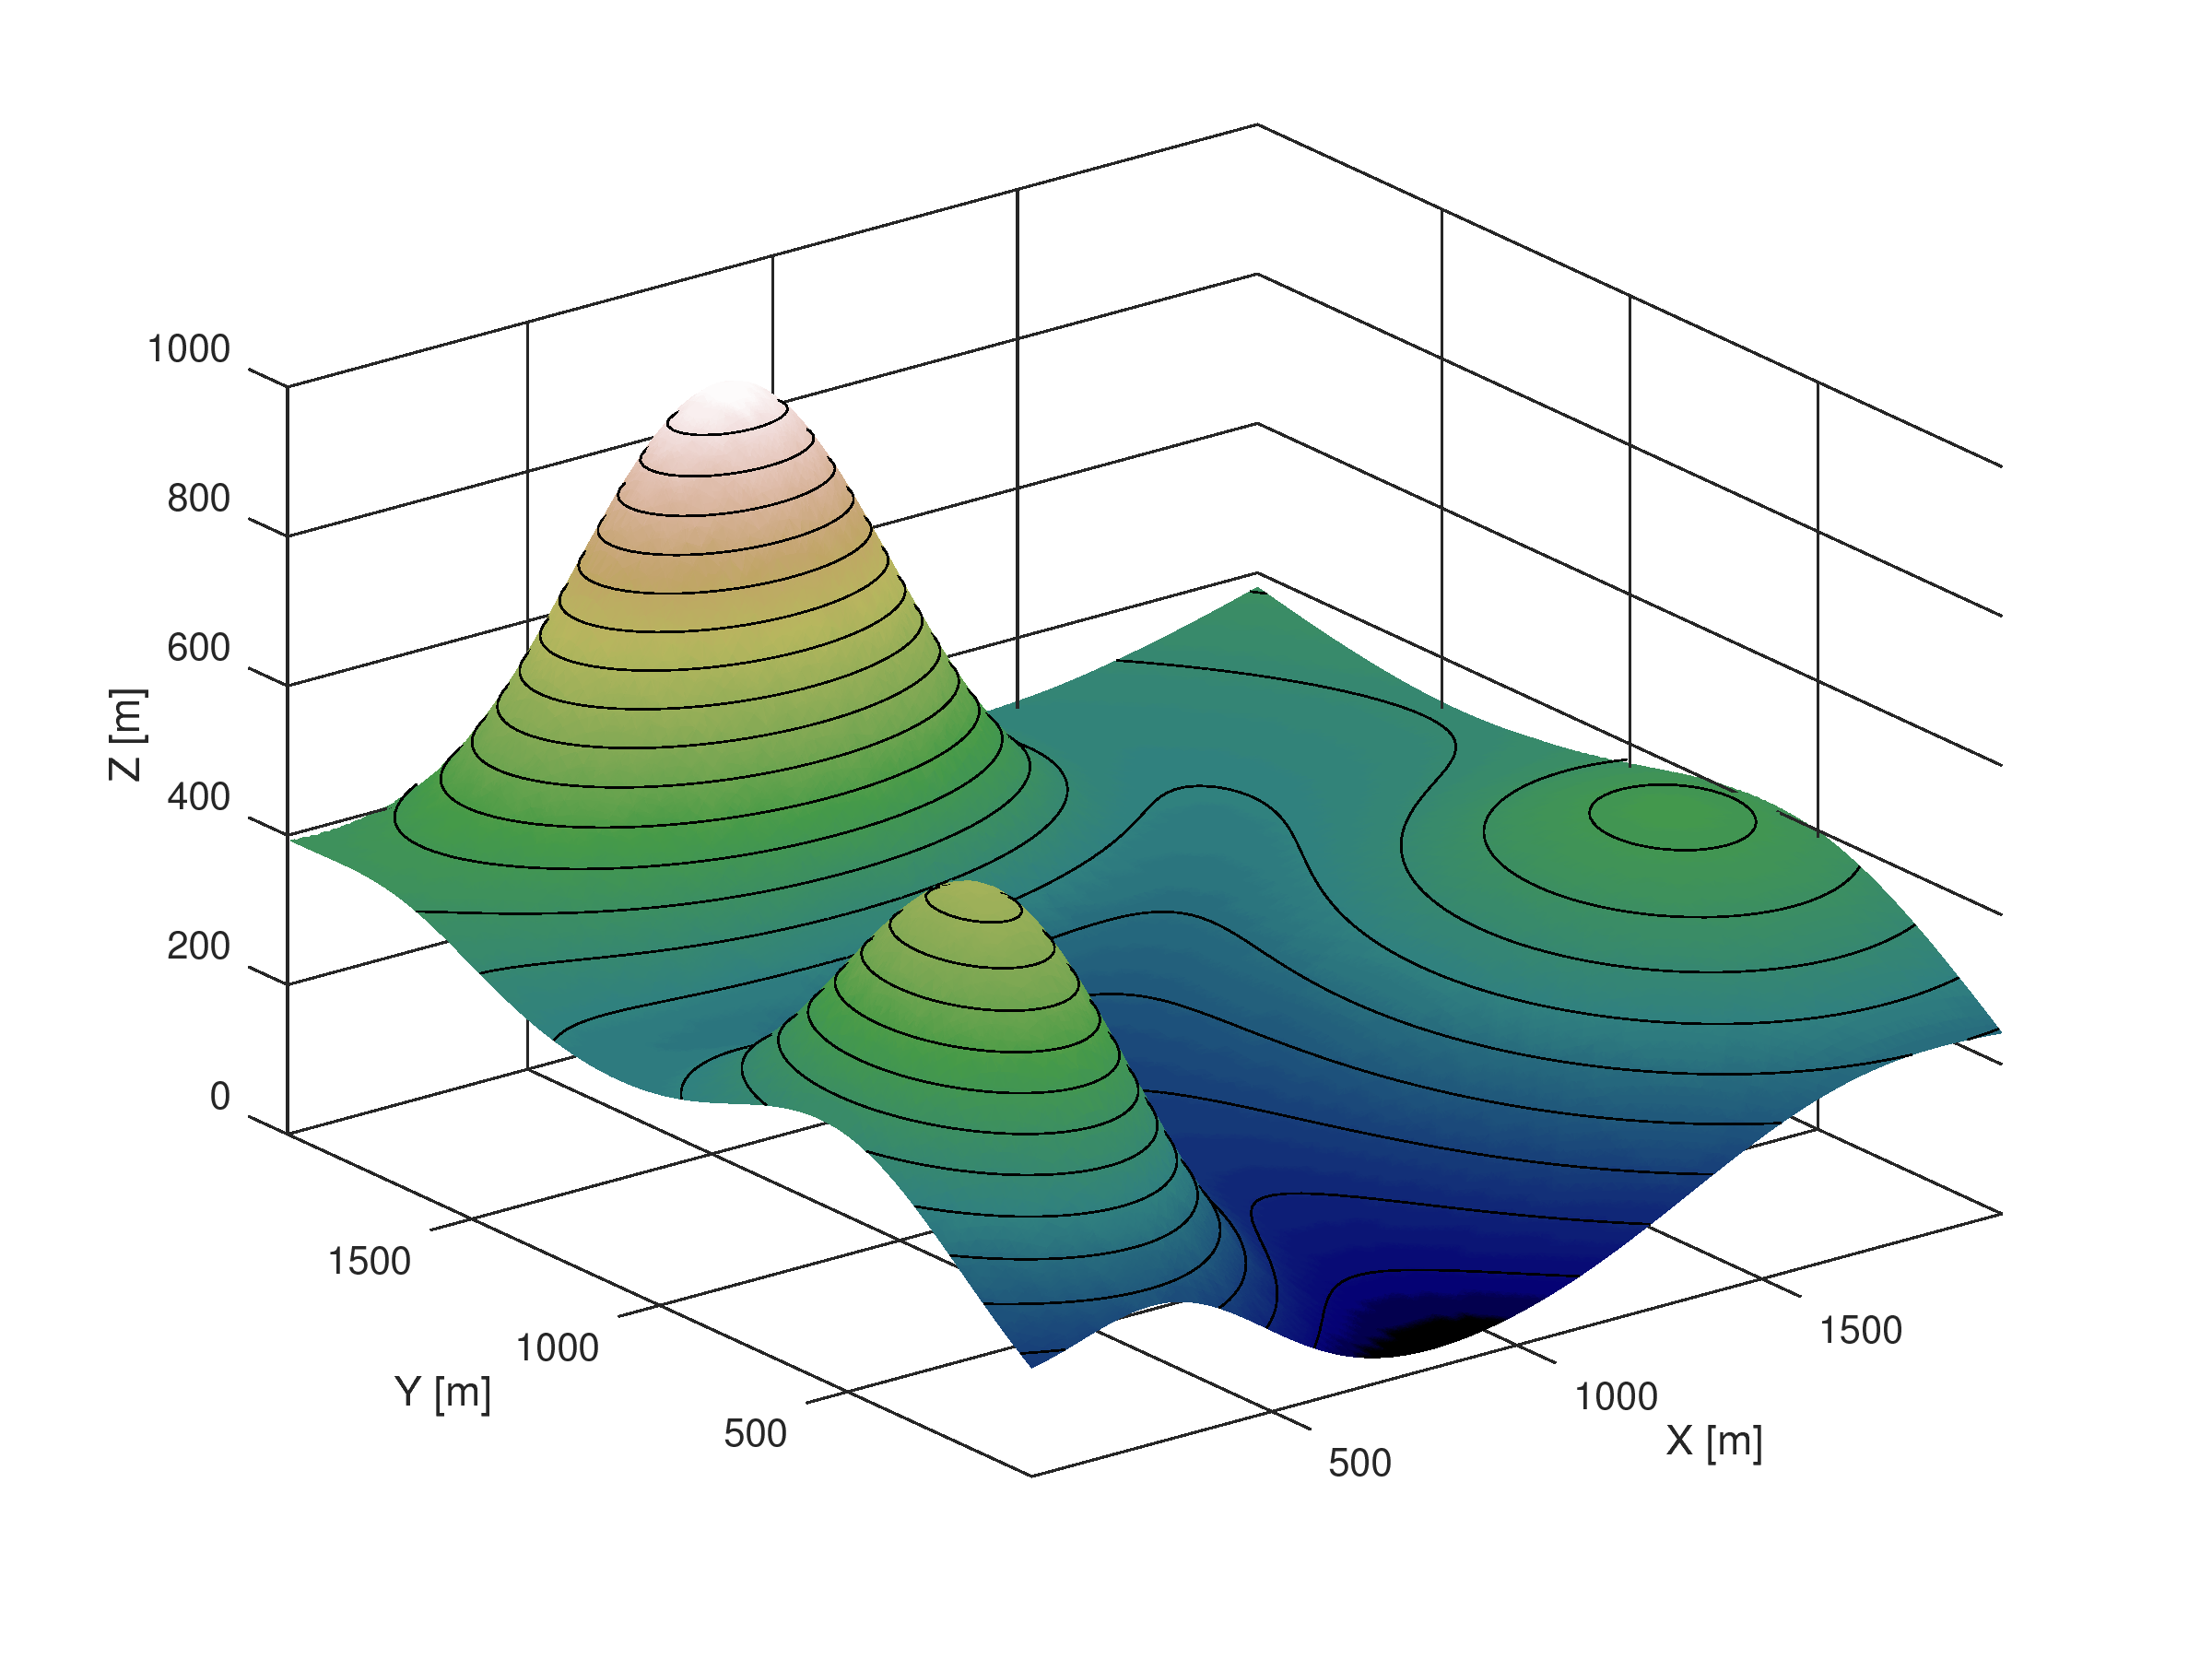
\includegraphics[width=0.7\textwidth]{Figures/topography.png}
  \caption{Synthetic topography composed of three Gaussian bumps on a sloping plane.}
  \label{fig:topography}
\end{figure}


\subsubsection{Setting-up the simulations}

The dataset required for building the emulator was generated by running \num{50} simulations with different combinations of the variables \emph{rain intensity} ($I$) and \emph{initial soil saturation} ($\theta_i$).
The initial soil saturation, being a spatially distributed variable, was kept uniform over the whole domain.
The rain intensity was kept constant and was uniformly applied over the domain, also since \textit{FullSWOF\_2D}, at this stage of development, only allows for uniformly distributed rain events \autocite{laguerre_documentation_2016}.

\num{5} different initial saturations in the $[\numrange{0}{1}]$ interval and \num{10} rain intensities in the \SIrange{10}{35}{\milli\metre\per\hour} interval were taken and all their possible combinations were used as inputs for the simulations.
The rain duration was set to \SI{6}{\hour}, while a simulation duration of \SI{9}{\hour} was chosen in order to be able to observe the hydrograph recession. A time resolution of \SI{60}{\second} was used, which means that intermediate simulation results were written to the \emph{outputs} file every \SI{60}{\second}.

Some parameters, namely those specific for the catchment in questions, were kept constant over all of the simulations.
These are summarized in Tab.~\ref{tab:simulations_parameters}.
The parameters marked with * are those \emph{spatially distributed}, meaning that a different value could be set for every cell.
For simplicity, a spatially uniform catchment was used, therefore the values from the table are valid for the whole domain.
Three \textit{wall boundary conditions} were set, for the upper and the two lateral boundaries.
For the bottom boundary a \textit{Neumann boundary condition} was selected, allowing water to freely outflow through that boundary and making sure that all of the water is lost from here.

\begin{table}[htpb]
  \centering
  \caption{Parameters and setting fixed for all simulations.}
  \label{tab:simulations_parameters}
  \begin{threeparttable}
    \begin{tabular}{lrl}
      \toprule
      \textbf{Parameter} & \textbf{Value} & \textbf{Units} \\
      \midrule
      Domain x-length                          &    $2'000$           & \si{\meter}   \\
      Domain y-length                          &    $2'000$           & \si{\meter}   \\
      Number of cells x                        &    $100$             & --   \\
      Number of cells y                        &    $100$             & --   \\
      Friction coefficient\tnote{*}            &    $0.03$            & \si{s.m^{-1/3}}\\
      Crust thickness\tnote{*}                 &    $1$               & \si{\meter}\\
      Crust hydraulic conductivity\tnote{*}    &    $2\cdot 10^{-6}$  & \si{\meter\per\second}\\
      Soil hydraulic conductivity\tnote{*}     &    $2\cdot 10^{-6}$  & \si{\meter\per\second}\\
      Soil suction head\tnote{*}               &    $0.09$      & \si{\meter}\\
      Soil maximum infiltration rate\tnote{*}  &    $19.8$      & \si{\milli\meter\per\hour}\\
      \bottomrule
    \end{tabular}
    \begin{tablenotes}
      \item[*] Parameters spatially distributed.
    \end{tablenotes}
  \end{threeparttable}
\end{table}


\subsubsection{Extracting the datasets}

%This data constitute the \emph{training} dataset for the emulator.
%A \emph{test} dataset and a \emph{validation} dataset were also generated and can be found in the Appendix~\ref{Appendix}. \noteseb{verify if they are really added}


The datasets used to build the emulator was extracted from the simulation outputs.
The extraction was done in two steps.
In the first step the outflow hydrographs were extracted from the output data. 
This was done by summing up the cell discharge along the whole domain bottom boundary for every saved time-step (one value every \SI{60}{\second}).
Result of this operation is a discharge values time series of \num{540} elements.
The same procedure was repeated with every one of the \num{50} experiments.
Fig.~\ref{fig:hydrographs3d} shows the extracted hydrographs.
Here many interesting features can be observed.
First of all it can be seen that experiments run with the two lowest rain intensities and low initial soil saturation generated no discharge.


\begin{figure}[htpb]
  \centering
  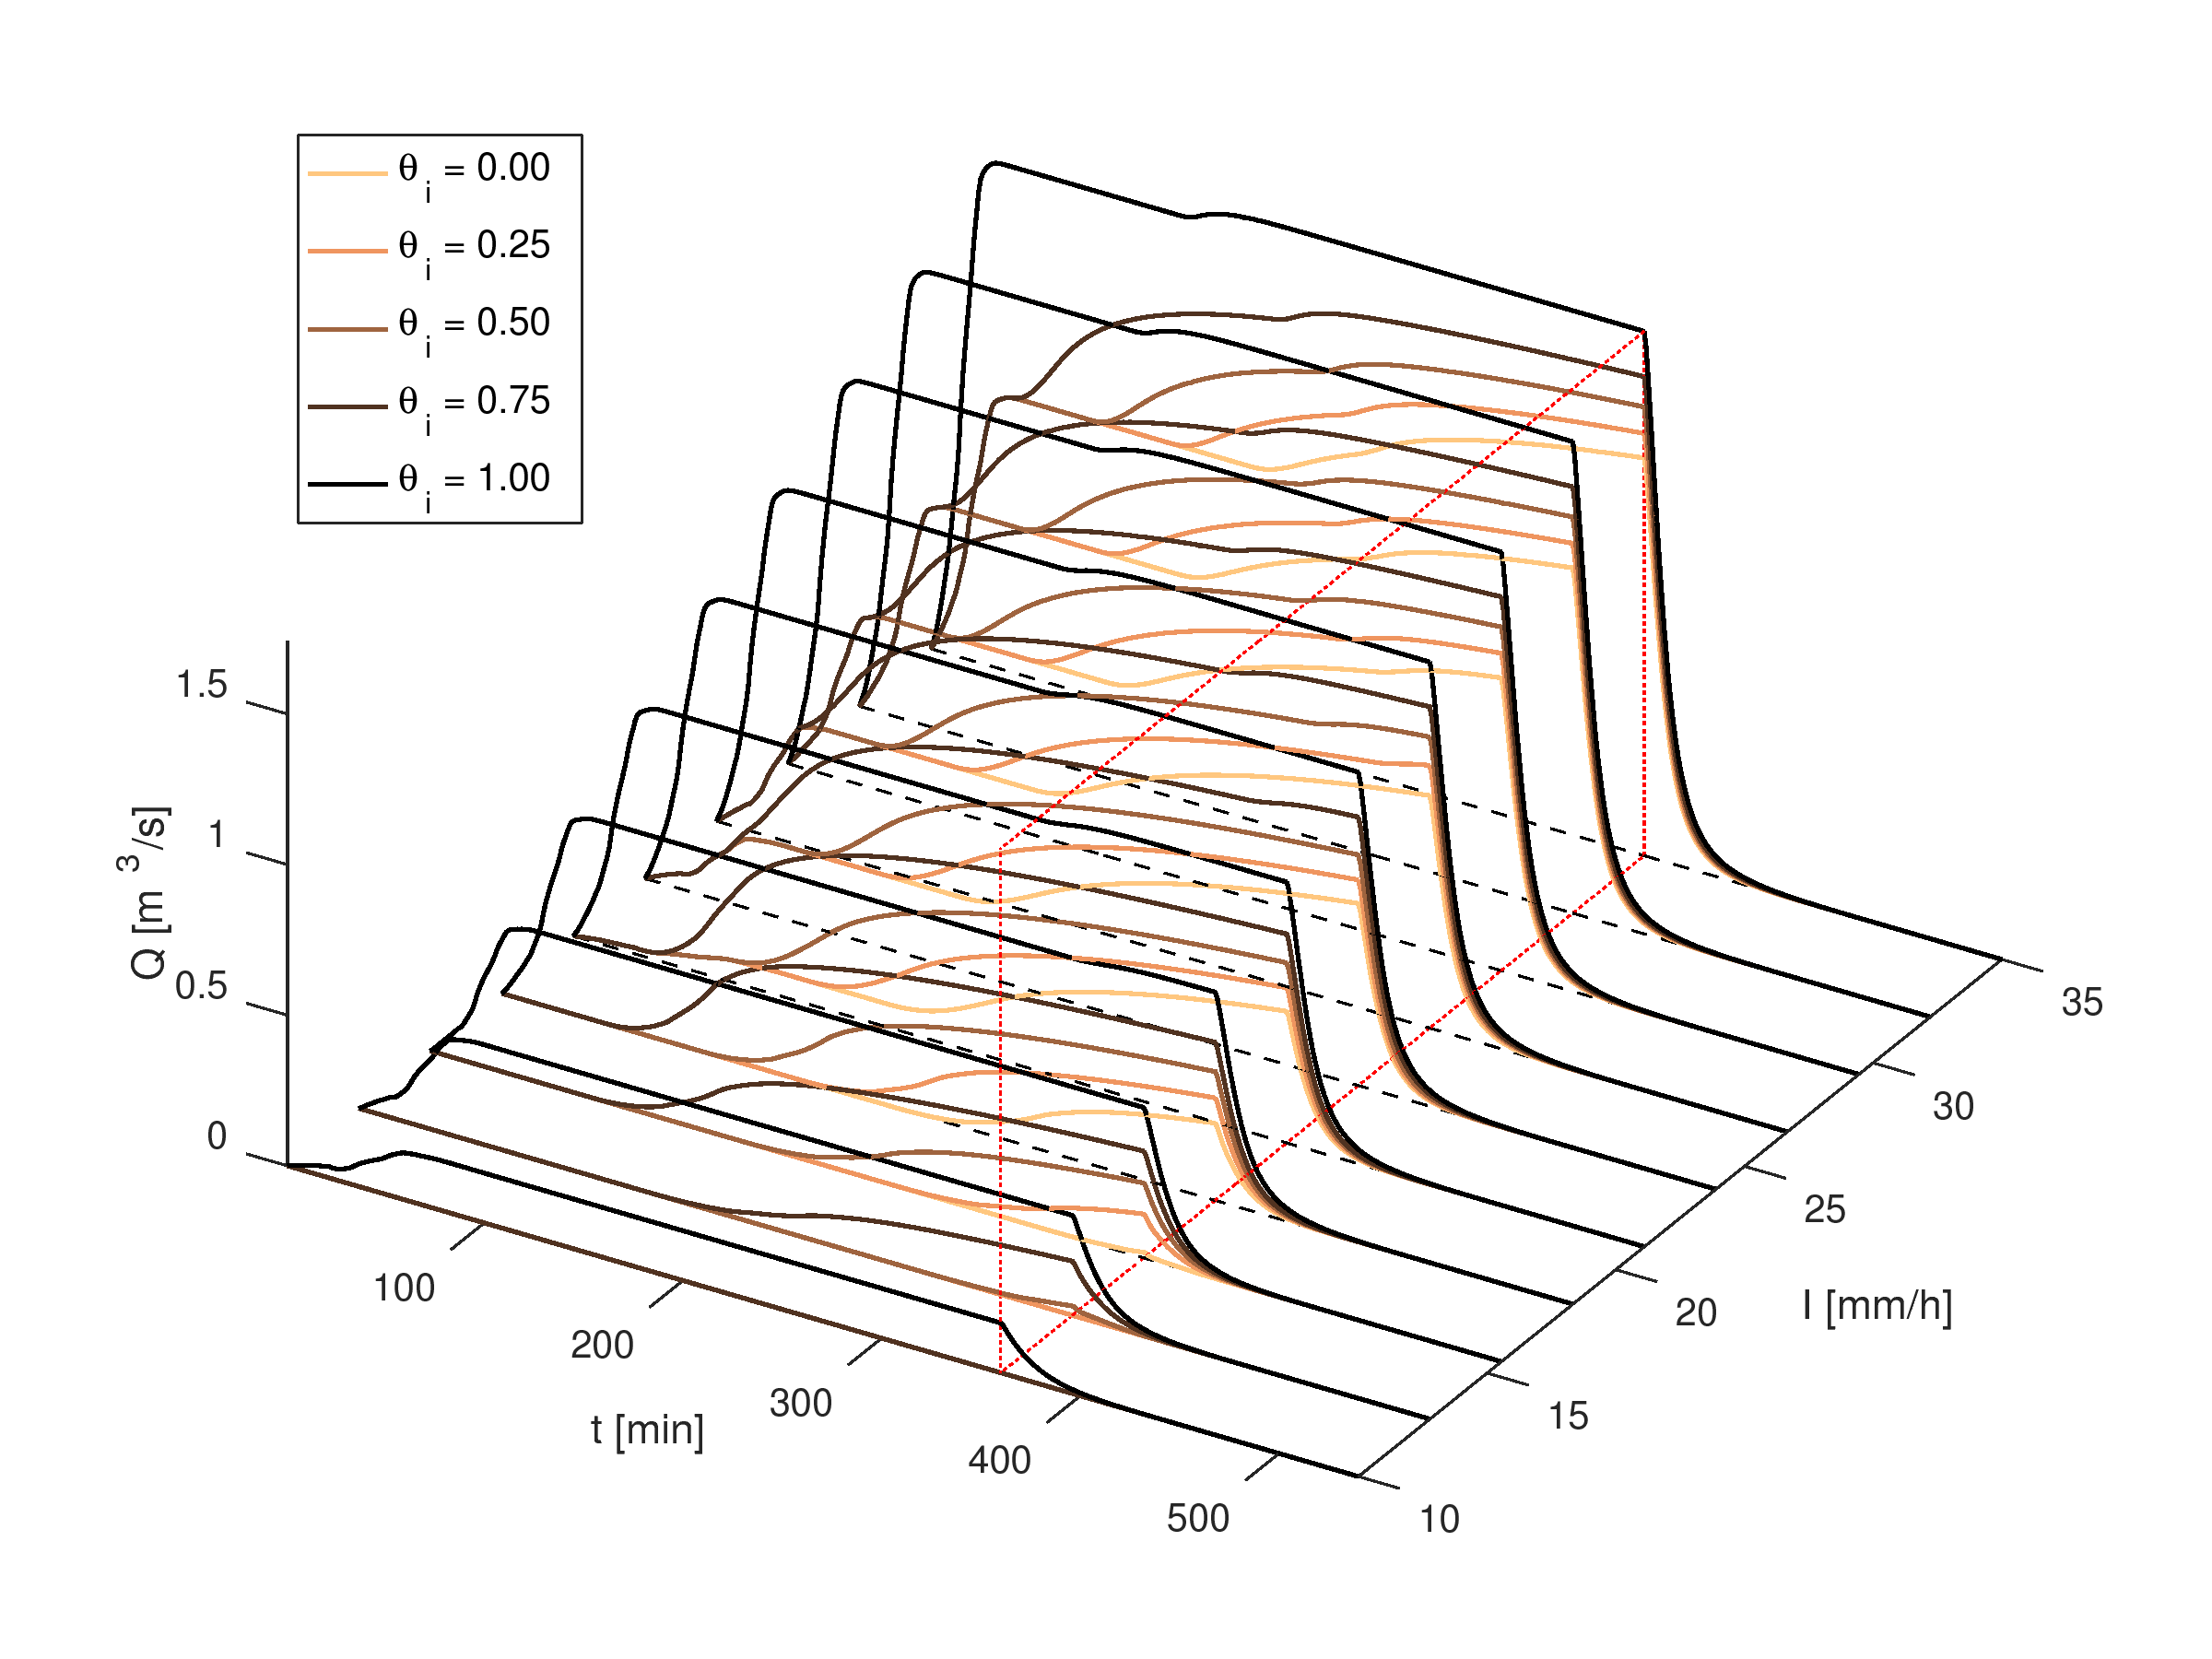
\includegraphics[width=0.75\textwidth]{Figures/hydrographs3d.png}
  \caption{Response hydrographs for the \num{50} simulations at the catchment outlet. The red frame shows the end of the rain event. Depth-dimension shows the \emph{rain intensity} variable, while the \emph{initial saturation} variable is rendered by the colormap.}
  \label{fig:hydrographs3d}
\end{figure}


\subsubsection{Building-up the classification emulator}


\subsubsection{Building-up the regression emulator}


% ---------------------------------------------------------------------------------------------------
\subsection{Results and discussion}
% ---------------------------------------------------------------------------------------------------

\begin{itemize}
\itemsep0em
  \item emulator should never underestimate danger (what type of error is this? we want to avoid it absolutely)
  \item try to perform GP interpolation. If it does not work, explain why polynomial interpolation (no time)
  \item use emulator with uncertainty in the $I$ and $\theta_i$. Perform uncertainty quantification
\end{itemize}


\subsubsection{Classification emulator}

Results for the classification emulator
\begin{itemize}
  \item show classification with 3 different $Q_!$
  \item perform testing 
\end{itemize}

\begin{figure}[htpb]
  \centering
  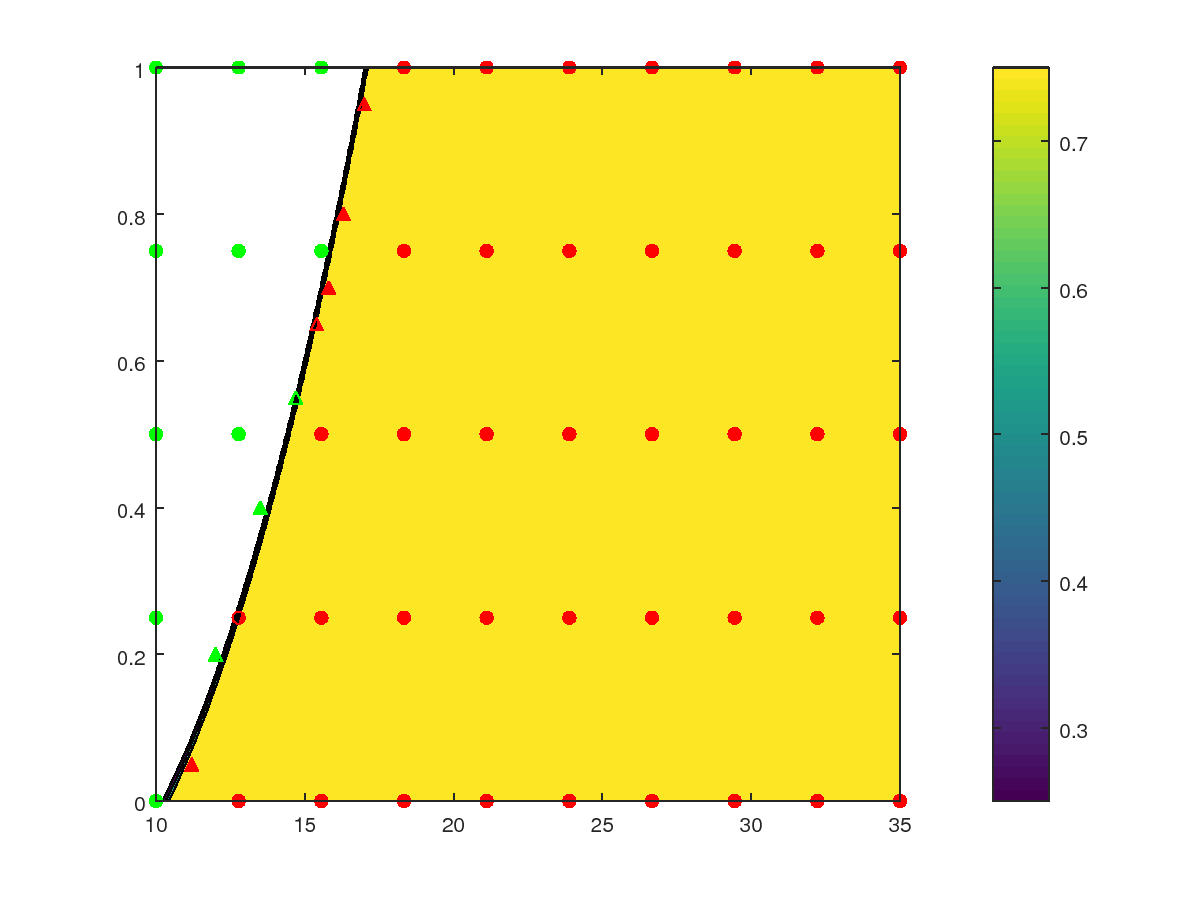
\includegraphics[width=0.75\textwidth]{Figures/classification.png}
  \caption{Binary classification emulator: events reaching $Q_!$ (red) and events not reaching $Q_!$ (green) for $Q_! = XX.X$.}
  \label{fig:classification_Q1}
\end{figure}


\subsubsection{Regression emulator}

\begin{figure}[htpb]
  \centering
  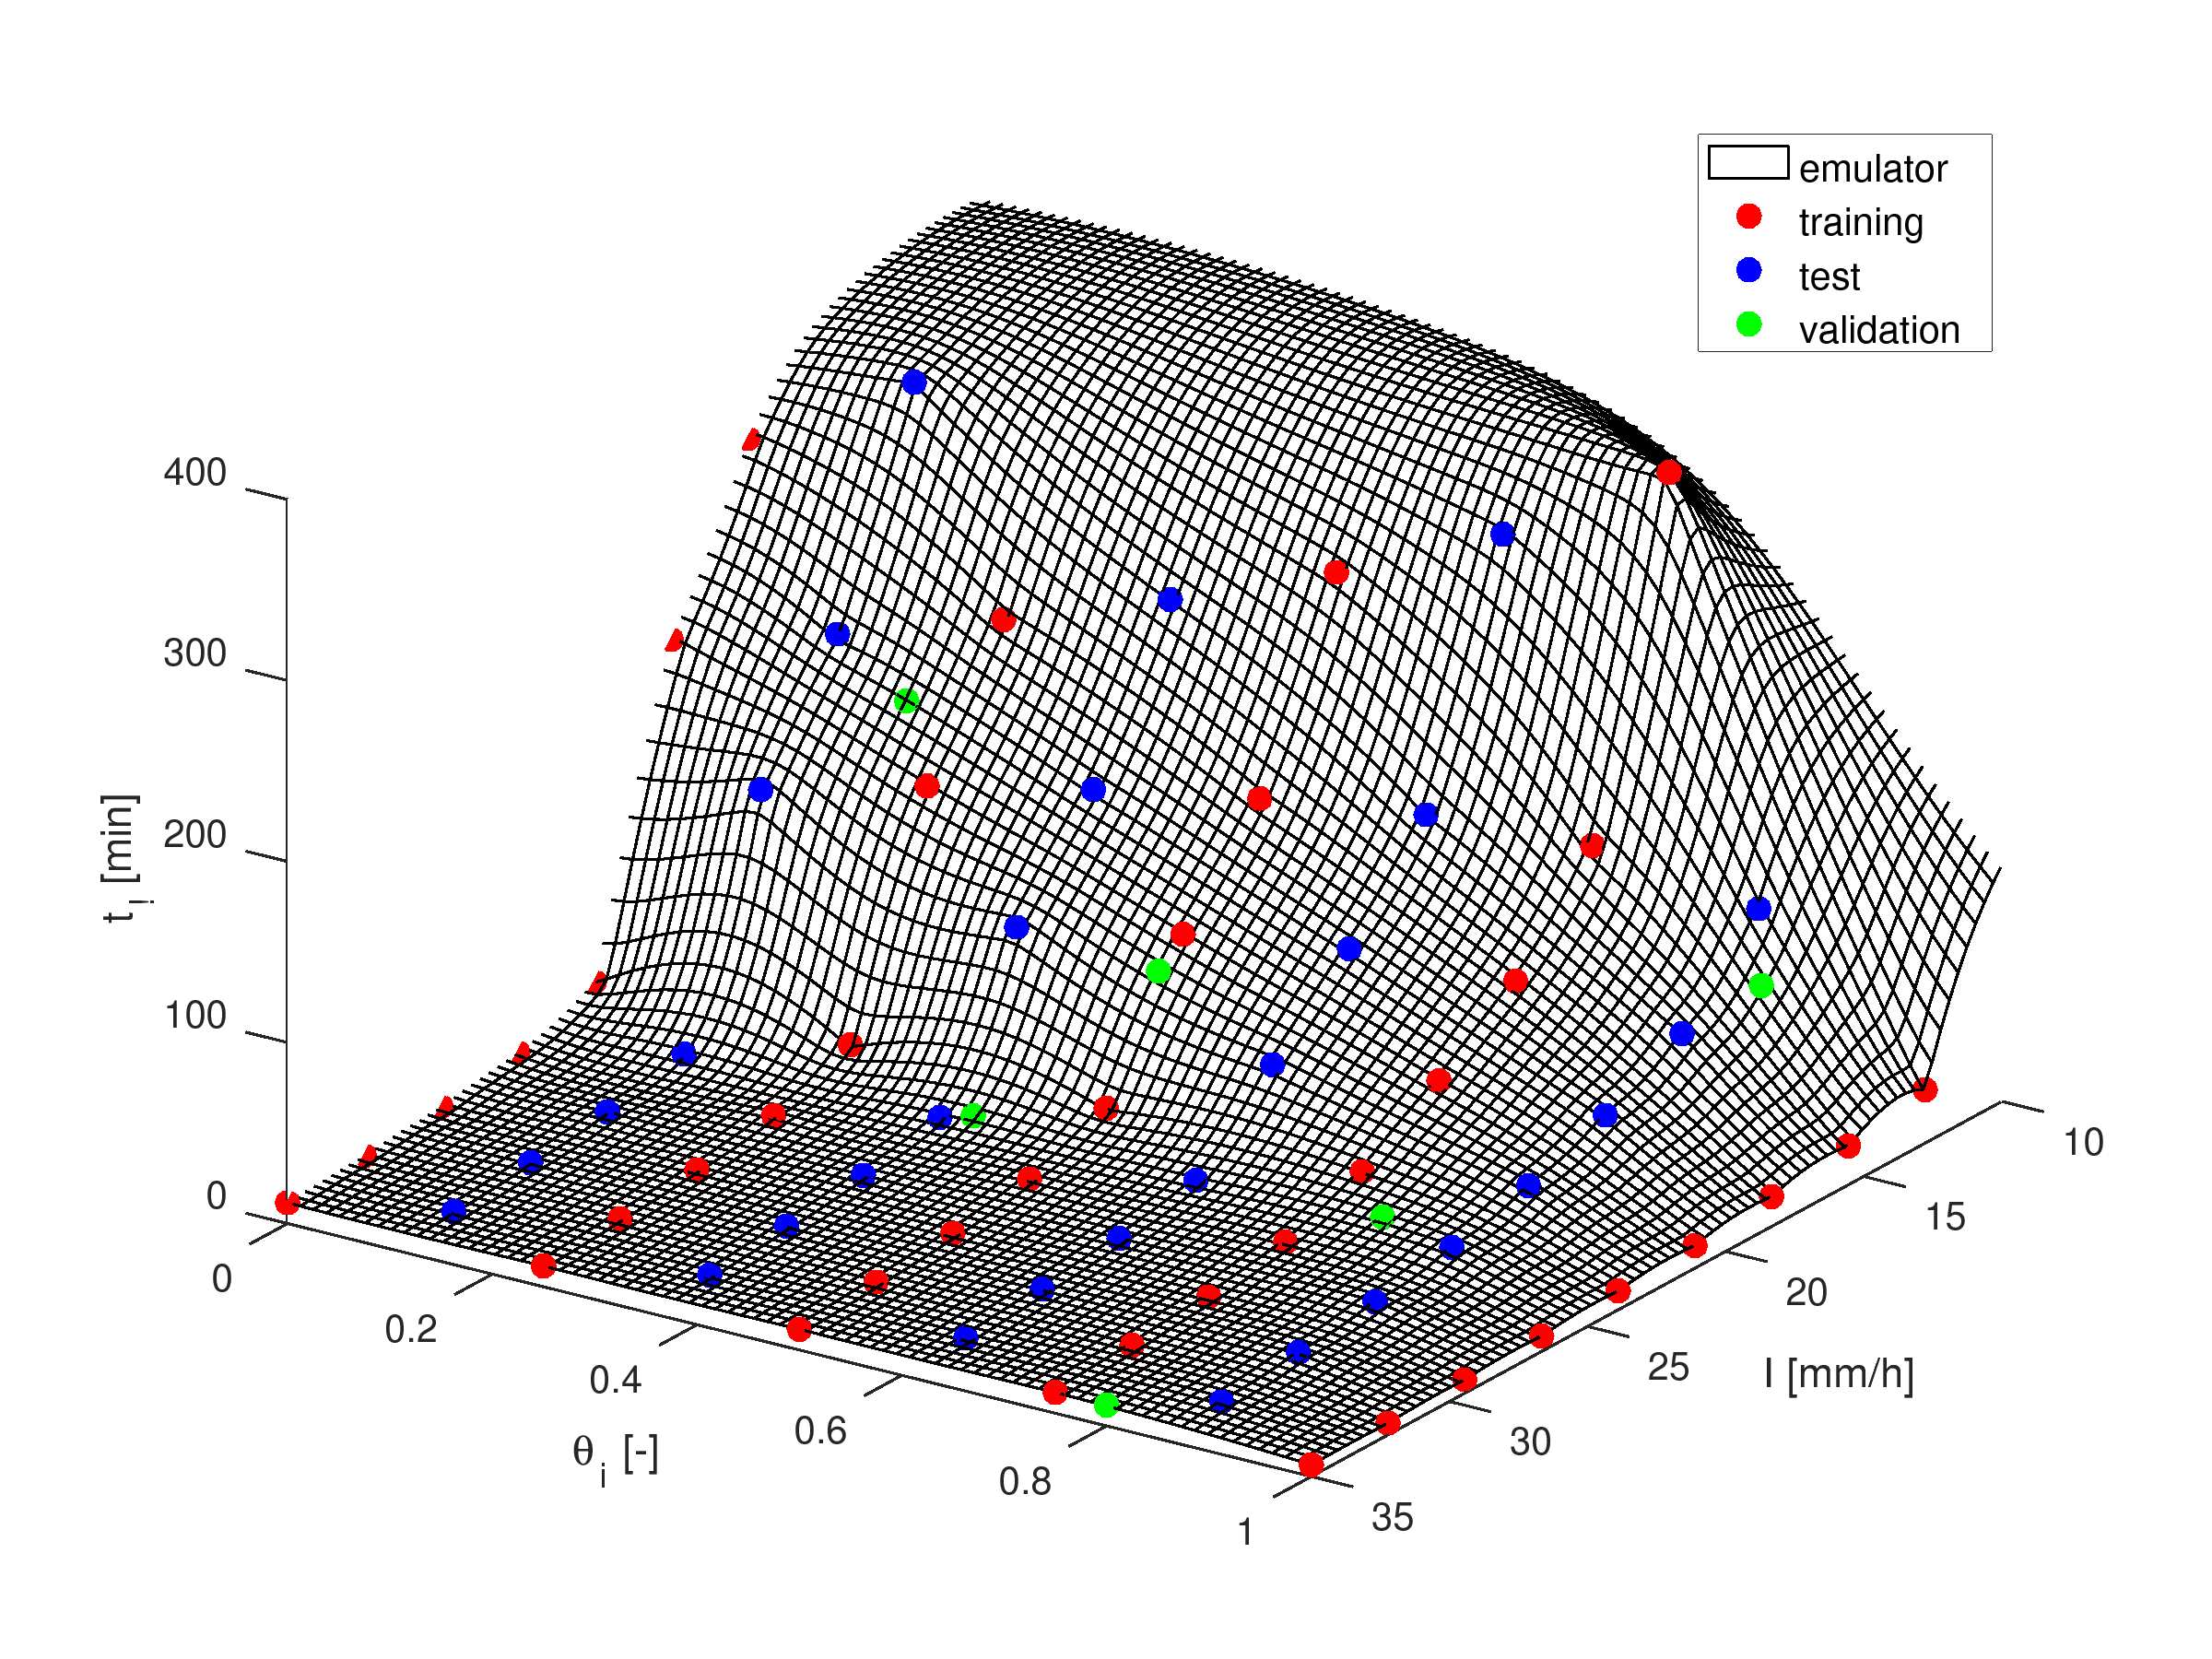
\includegraphics[width=0.7\textwidth]{Figures/emulator.png}
  \caption{Time-to-threshold emulator: training (red), test (blue) and validation (green) datasets and the emulator producing the intrapolation response.}
  \label{fig:regression_emulator}
\end{figure}


\begin{table}[htpb]
  \centering
  \caption{Emulator performance on \emph{test} and \emph{validation} data}
  \label{table label}
  \begin{tabular}{lcc}
    \toprule
     & \textbf{MAE [\si{\minute}, \si{\percent}]} & \textbf{RMSE [\si{\minute}, \si{\percent}]} \\
    \midrule
    \textbf{test} & val & val \\
    \textbf{validation} & val & val \\
    \bottomrule
  \end{tabular}
\end{table}

